\documentclass[12pt,a4paper]{article}
\usepackage[utf8]{inputenc}
\usepackage{amsmath}
\usepackage{amsfonts}
\usepackage{amssymb}
\usepackage[brazil]{babel}
\usepackage{indentfirst}
\usepackage{url}
\usepackage{float}
\usepackage{color}
\usepackage{colortbl}

\definecolor{pblue}{rgb}{0.13,0.13,1}
\definecolor{pgreen}{rgb}{0,0.5,0}
\definecolor{pred}{rgb}{0.9,0,0}
\definecolor{pgrey}{rgb}{0.46,0.45,0.48}
\usepackage{listings}
\lstset{language=SQL,
  showspaces=false,
  showtabs=false,
  breaklines=true,
  showstringspaces=false,
  breakatwhitespace=true,
  commentstyle=\color{pgreen},
  keywordstyle=\color{pblue},
  stringstyle=\color{pred},
  basicstyle=\ttfamily,
  moredelim=[il][\textcolor{pgrey}]{\$\$},
  moredelim=[is][\textcolor{pgrey}]{\%\%}{\%\%}
}
%%%%%%%%%%%%%%%%%%%%%%%%%%%%%%%%Fim codigo JAVA%%%%%%%%%%%%%%
%%%%%%%%%%%Codigo geral%%%%%%%%%%%%%%%%%%%%%%%%%%%%%%%%%%%%%%
\definecolor{mygreen}{rgb}{0,0.6,0}
\definecolor{mygray}{rgb}{0.5,0.5,0.5}
\definecolor{mymauve}{rgb}{0.58,0,0.82}
\lstset{ %
  backgroundcolor=\color{white},   % choose the background color; you must add \usepackage{color} or \usepackage{xcolor}; should come as last argument
  basicstyle=\footnotesize,        % the size of the fonts that are used for the code
  breakatwhitespace=false,         % sets if automatic breaks should only happen at whitespace
  breaklines=true,                 % sets automatic line breaking
  captionpos=b,                    % sets the caption-position to bottom
  commentstyle=\color{mygreen},    % comment style
  deletekeywords={...},            % if you want to delete keywords from the given language
  escapeinside={\%*}{*)},          % if you want to add LaTeX within your code
  extendedchars=true,              % lets you use non-ASCII characters; for 8-bits encodings only, does not work with UTF-8
  frame=single,                    % adds a frame around the code
  keepspaces=true,                 % keeps spaces in text, useful for keeping indentation of code (possibly needs columns=flexible)
  keywordstyle=\color{blue},       % keyword style
  language=Octave,                 % the language of the code
  morekeywords={*,...},            % if you want to add more keywords to the set
  numbers=left,                    % where to put the line-numbers; possible values are (none, left, right)
  numbersep=5pt,                   % how far the line-numbers are from the code
  numberstyle=\tiny\color{mygray}, % the style that is used for the line-numbers
  rulecolor=\color{black},         % if not set, the frame-color may be changed on line-breaks within not-black text (e.g. comments (green here))
  showspaces=false,                % show spaces everywhere adding particular underscores; it overrides 'showstringspaces'
  showstringspaces=false,          % underline spaces within strings only
  showtabs=false,                  % show tabs within strings adding particular underscores
  stepnumber=1,                    % the step between two line-numbers. If it's 1, each line will be numbered
  stringstyle=\color{mymauve},     % string literal style
  tabsize=2,                       % sets default tabsize to 2 spaces
  title=\lstname                   % show the filename of files included with \lstinputlisting; also try caption instead of title
}

\RequirePackage{graphicx}
\title{Dicionário de Dados}
\author{Daniel Moreira Cardoso \and Gusttavo Nunes Gomes\and Ianka Talita Bastos de Assis\and Ígor Justino Rodrigues \and Thalia Santos de Santana}
\usepackage[left=3cm,right=3cm,top=2cm,bottom=2cm]{geometry}
\begin{document}
\begin{titlepage}
\begin{center}
\begin{figure}[htb]
	\label{figura:LogoIF}
	\centering
	
\includegraphics[width=6cm]{recursos/imagens/logo.png} 
\end{figure}
Instituto Federal Goiano - Campus Ceres\\
Bacharelado em Sistemas de Informação\\
Prof. Me. Ronneesley Moura Teles\\\vspace{1cm}

Daniel Moreira Cardoso \\ 
Gusttavo Nunes Gomes \\ 
Ianka Talita Bastos de Assis \\ 
Ígor Justino Rodrigues \\ 
Thalia Santos de Santana\\
\vspace{6.0cm}
\textit{\textbf{\Large{Diferenças de desempenho do uso de BLOBs no banco de dados}}}\\\vspace{10cm}
Novembro\\
2017\\
\end{center}
\end{titlepage}
\tableofcontents
\newpage
\begin{center}
\textbf{\Large{Diferenças de desempenho do uso de BLOBs no banco de dados}}\\\vspace{0.5cm}
\end{center}
\section{Introdução}
O BLOB \textit{(Binary Large Object)}, ou em português, Grande Objeto Binário, refere-se a campos criados para armazenar qualquer tipo de informação em formato binário, dentro de um banco de dados [1]. Geralmente, são arquivos multimídia, como imagens, áudios, vídeos, etc. Normalmente, grande parte dos bancos de dados (BDs) dão suporte aos tipos básicos, como datas, \textit{strings}, números e assim, para aqueles que não fazem parte dessa linha, utiliza-se BLOBs [2].

O MySQL também faz uso de BLOBs e são divididos em quatro tipos [1]:
\begin{itemize}
	\item TINYBLOB: campo BLOB de armazenamento máximo igual a 255 caracteres (8 bits) mais 1 de controle;
	\item BLOB: o mesmo que o Tinyblob, porém armazenando até 16535 caracteres (16 bits) mais 2 de controle;
	\item MEDIUMBLOB: o mesmo que o Tinyblob, porém armazenando até 16777216 caracteres (24 bits) mais 3 de controle;
	\item LONGBLOB: o mesmo que o Tinyblob, porém armazenando até 4294967295 caracteres (32 bits) mais 4 de controle.
\end{itemize}

De acordo com o site \textit{ITPro}, trabalhar com armazenamento de dados usando BLOB faz com que todas as informações se mantenham em uma entidade de maneira conjunta, o que acarreta em facilidades de busca e de recuperação de dados. Mas infelizmente, isso acaba gerando um banco de dados com tamanho elevado [3]. 

Quando trata-se de armazenar separadamente, com uso de URLs (Localizador Uniforme de Recursos), os bancos são menores comparativamente, além de trazer rapidez, pois o processo de leitura de dados sobrecarrega muito menos do que ler no próprio BD. Mas é necessário sempre realizar mantenimento manual do \textit{link}, ao qual, liga o BD e o arquivo externo [3].

O autor ainda afirma que é possível guardar arquivos binários fora do BD e incluí-los como URL para o objeto, unindo as técnicas apresentadas.

Em alguns fóruns, como \textit{yiiframework}, alguns participantes sugerem BLOBs devido ao quesito segurança. Porém, no quesito desempenho, os mesmos concordam que URL é a melhor forma de trabalho. Outro correspondente afirma, inclusive, que essa escolha deve depender de como aplicação é estruturada, mas ele prefere fazer uso de caminhos do arquivo [4].

Já no \textit{Stack Exchange}, há concordância que depende do caso específico. Para um dos usuários, BLOBs traz gerenciabilidade, ajudando em situações que envolvam restauração do BD e \textit{backups} [5]. 

Segundo ainda o Blog \textit{SQL Authority}, a autor faz a sugestão em prol do armazenamento da localização das imagens (por exemplo), no banco de dados usando o tipo de dados VARCHAR em vez de qualquer BLOB ou outro tipo de dados binário. Sua explicação está ligada ao fato de que armazenar a localização ao invés do BLOB reduz muito o tamanho do BD, bem como atualizar ou substituir a imagem são métodos mais simples, visto que refere-se apenas a uma operação de arquivo em vez de uma atualização efetiva de \textit{inserts} e \textit{delets} no BD [6].

Ademais, há um artigo intitulado \textit{``To BLOB or Not To BLOB: Large Object Storage in a Database or a Filesystem?''} [7], que descreve que ao realizar a decisão por se armazenar em um sistema de arquivos ou em uma base de dados, é feita através de atributos como simplicidade de aplicação ou capacidade de gerenciamento, sabendo que o desempenho do sistema acaba afetando esses fatores. Os autores recordam que é de conhecimento que BDs lidam eficientemente com
grande número de objetos pequenos, enquanto sistemas de arquivos são mais eficiente para objetos grandes. O estudo traz a informação que BLOBs menores do que 256KB são mais eficientemente gerenciados por um BD, enquanto um sistema de arquivos é mais eficiente para aqueles maiores do que 1 MB, com variações decorrentes de diferentes BDs e sistemas de arquivos.

Além disso, os mesmos afirmam que o desempenho muda ao longo do tempo conforme o armazenamento torna-se fragmentado, sendo este tema, parte importante das contextações do estudo, concentrando-se em problemas de fragmentação de armazenamento. Verifica-se que, em síntese, os sistemas de arquivos parecem ter uma melhor fragmentação e manipulação do que BDs e isso impulsiona o ponto de equilíbrio de cerca de 1 MB para aproximadamente 256KB.


\section{Aplicação}
Em busca de avaliar o desempenho do uso de BLOBs, criou-se a mesma tabela (Figura 1), uma contendo o BLOB e outra com a URL do arquivo.

\begin{figure}[htb]
	\label{figura:tabelas}
	\centering
	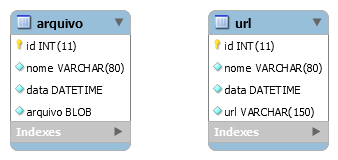
\includegraphics[width=8cm]{recursos/imagens/tabelas.png} 
	
	Figura 1. Tabela com uso de BLOB e tabela com URL.
\end{figure}

Em cada uma das tabelas foram inseridos 49000 registros, igualmente. A partir destes, avaliou-se a diferença de tempo de 1000 consultas. Abaixo, tem-se o arquivo \textit{.sql} referente a criação das tabelas no SGBD (Sistema Gerenciador de Banco de Dados) \textit{MySQL Workbench}. \\\vspace{0.1cm}

\lstinputlisting[language=SQL]{recursos/codigos/banco.sql}

\section{Resultados}

Avaliando-se o desempenho, algumas consultas foram realizadas com 1000 repetições, selecionando por data, nome e por todos os campos, a qual essa última, informa se há ou não real diferença em relação ao uso de BLOBs. Todos os tempos de cada consulta foram salvos, gerando uma média final referente a cada \textit{select}. No caso do BLOB, o \textit{sql} retrata o uso de \textit{limit 100}, visto que o BD não conseguiu com lidar com os dados, e o máximo alcançado justamente trata-se de 100 registros por vez.
\\\vspace{0.1cm}

\lstinputlisting[language=SQL]{recursos/codigos/Select_Data_Blob.txt}

\lstinputlisting[language=SQL]{recursos/codigos/Select_Data_URL.txt}

\lstinputlisting[language=SQL]{recursos/codigos/Select_Nome_Blob.txt}

\lstinputlisting[language=SQL]{recursos/codigos/Select_Nome_URL.txt}

\lstinputlisting[language=SQL]{recursos/codigos/Select_Todos_Blob.txt}

\lstinputlisting[language=SQL]{recursos/codigos/Select_Todos_URL.txt}

\section{Considerações finais}
Levando em conta o objetivo deste, ao realizar a comparação de desempenho nas consultas, fica claro que ao fazer uso de URLs, há maior rapidez nas consultas do que usando BLOBs (0.1783877 seg $<$ 1.35309537 seg).



\section{Referências Bibliográficas}
\noindent \textbf{[1]} {https://pt.stackoverflow.com/questions/100802/como-funciona-o-campo-blob}\\\vspace{0.2cm}

\noindent \textbf{[2]} {https://pt.wikipedia.org/wiki/BLOB}\\\vspace{0.2cm}

\noindent \textbf{[3]} {http://www.itprotoday.com/cloud-data-center/storing-blobs-database-or-file-system}\\\vspace{0.2cm}

\noindent \textbf{[4]} {http://www.yiiframework.com/forum/index.php/topic/33244-best-practice-to-store-images-in-database-blob-or-url-based/}\\\vspace{0.2cm}

\noindent \textbf{[5]} {https://dba.stackexchange.com/questions/736/is-it-better-to-store-images-in-a-blob-or-just-the-url}\\\vspace{0.2cm}

\noindent \textbf{[6]} {https://blog.sqlauthority.com/2007/12/13/sql-server-do-not-store-images-in-database-store-location-of-images-url/}\\\vspace{0.2cm}

\noindent \textbf{[7]} SEARS, Russell; VAN INGEN, Catharine; GRAY, Jim. \textbf{To blob or not to blob: Large object storage in a database or a filesystem?.} arXiv preprint cs/0701168, 2007.

\end{document}

%\lstinputlisting[language=SQL]{recursos/codigo/01.sql}

%\lstinputlisting[language=SQL, firstline=3, lastline=5]{recursos/codigo/01.sql}

%%Modelo de código para inserir figura
%\begin{figure}[h]
%\centering
%
\includegraphics[width=15cm]{logo.png}
%\label{4}
%\caption{Fonte:http://...; Acesso em 06/11/2017}
%\end{figure}